\chapter{Grundlagen}\label{chap:Grundlagen}
\section{Susceptible-Infectious-Removed Modell}
Ein Weg zur Beschreibung der Pandemie bietet das SIR Modell \autocite{SIR}. Dieses Modell teilt die Mitglieder einer Menschengruppe in eine der drei folgenden Kategorie ein und ermöglicht es, die zeitliche Entwicklung einer Pandemie übersichtlich darzustellen:
\begin{itemize}
    \item \glqq{}susceptible\grqq{}: Menschen, welche angesteckt werden können.
    \item \glqq{}infectious\grqq{}: Infizierte Menschen, welche weitere Menschen anstecken können. Werden auch als "die aktiven Fälle" bezeichnet.
    \item \glqq{}recovered\grqq{}: Menschen, welche in die Kategorie \glqq{}infectious\grqq{} fielen und\\
    nun immun gegen die Krankheit sind. (Hierzu zählen auch Verstorbene)
\end{itemize}
Hierbei werden die Neuansteckungen ausgehend von einem infizierten Menschen mit der Reproduktionszahl $R$ beschrieben. Formal ist die Reproduktionszahl $R$ definiert durch die durchschnittliche Anzahl an infizierten Menschen pro Fall \autocite{ReZahl}.
%weitere Erklärung von R_0 siehe Fabians erste Einleitungsseite


\section{Korrelationsanalyse mithilfe einer Faltung}\label{sec:BeschreibungKorrelationsanalyse}
Um festzustellen, ob die sieben Tages Inzidenzen einiger Landkreise im Vergleich zu anderen Landkreisen eher voraus- oder nacheilen, wird in diesem Fall eine \glqq{}Faltung\grqq{} verwendet \autocite{Korrelation}.

Bei diskreten Werten aufgeteilt in zwei Zeitserien $X$ und $Y$, wie in diesem Fall, lässt sich eine Faltung sehr einfach umsetzen:
Für eine zeitliche Verschiebung $\tau$ wird mit jedem Wert $x_i$ zum jeweiligen Zeitpunkt $t_i$ aus der ersten Zeitserie mit dem zugehörigen Wert $y_i$ aus der zweiten Zeitserie eine Produkt gebildet. Der zugehörige Wert aus der zweiten Zeitserie entspricht hierbei dem Zeitpunkt $t$ des Wertes der ersten Zeitserie plus die gewählte Verschiebung $\tau$. Sollte dieser zweite Wert nicht existieren, wird kein Produkt gebildet.

Für jede zeitliche Verschiebung $\tau$, für die mindesten ein Produkt gebildet wird, werden alle möglichen Produkte aufsummiert.

Somit ergibt sich \autoref{eq:Korrelation}, mit $n := $ Länge von $X$ und wenn $y_{i+\tau} \not\in Y$, dann $y_{i+\tau} := 0$:
\begin{equation}\label{eq:Korrelation}
    c(\tau) = \sum_{i=1}^n x_i\cdot y_{i+\tau}
\end{equation}


Bildlich gesprochen wird die zweite Zeitserie an der ersten Zeitserie vorbeigeschoben, beginnend an dem Punkt, an dem ausschließlich das erste Element der ersten Zeitserie mit dem letzten Element der zweiten Zeitserie multipliziert wird. Dies ist beispielhaft mit den Folgen $[1,2,3,2]$ und $[5,7,5,1]$ in \autoref{fig:Korrelation Beispiel} dargestellt.

\begin{figure}
    \centering
    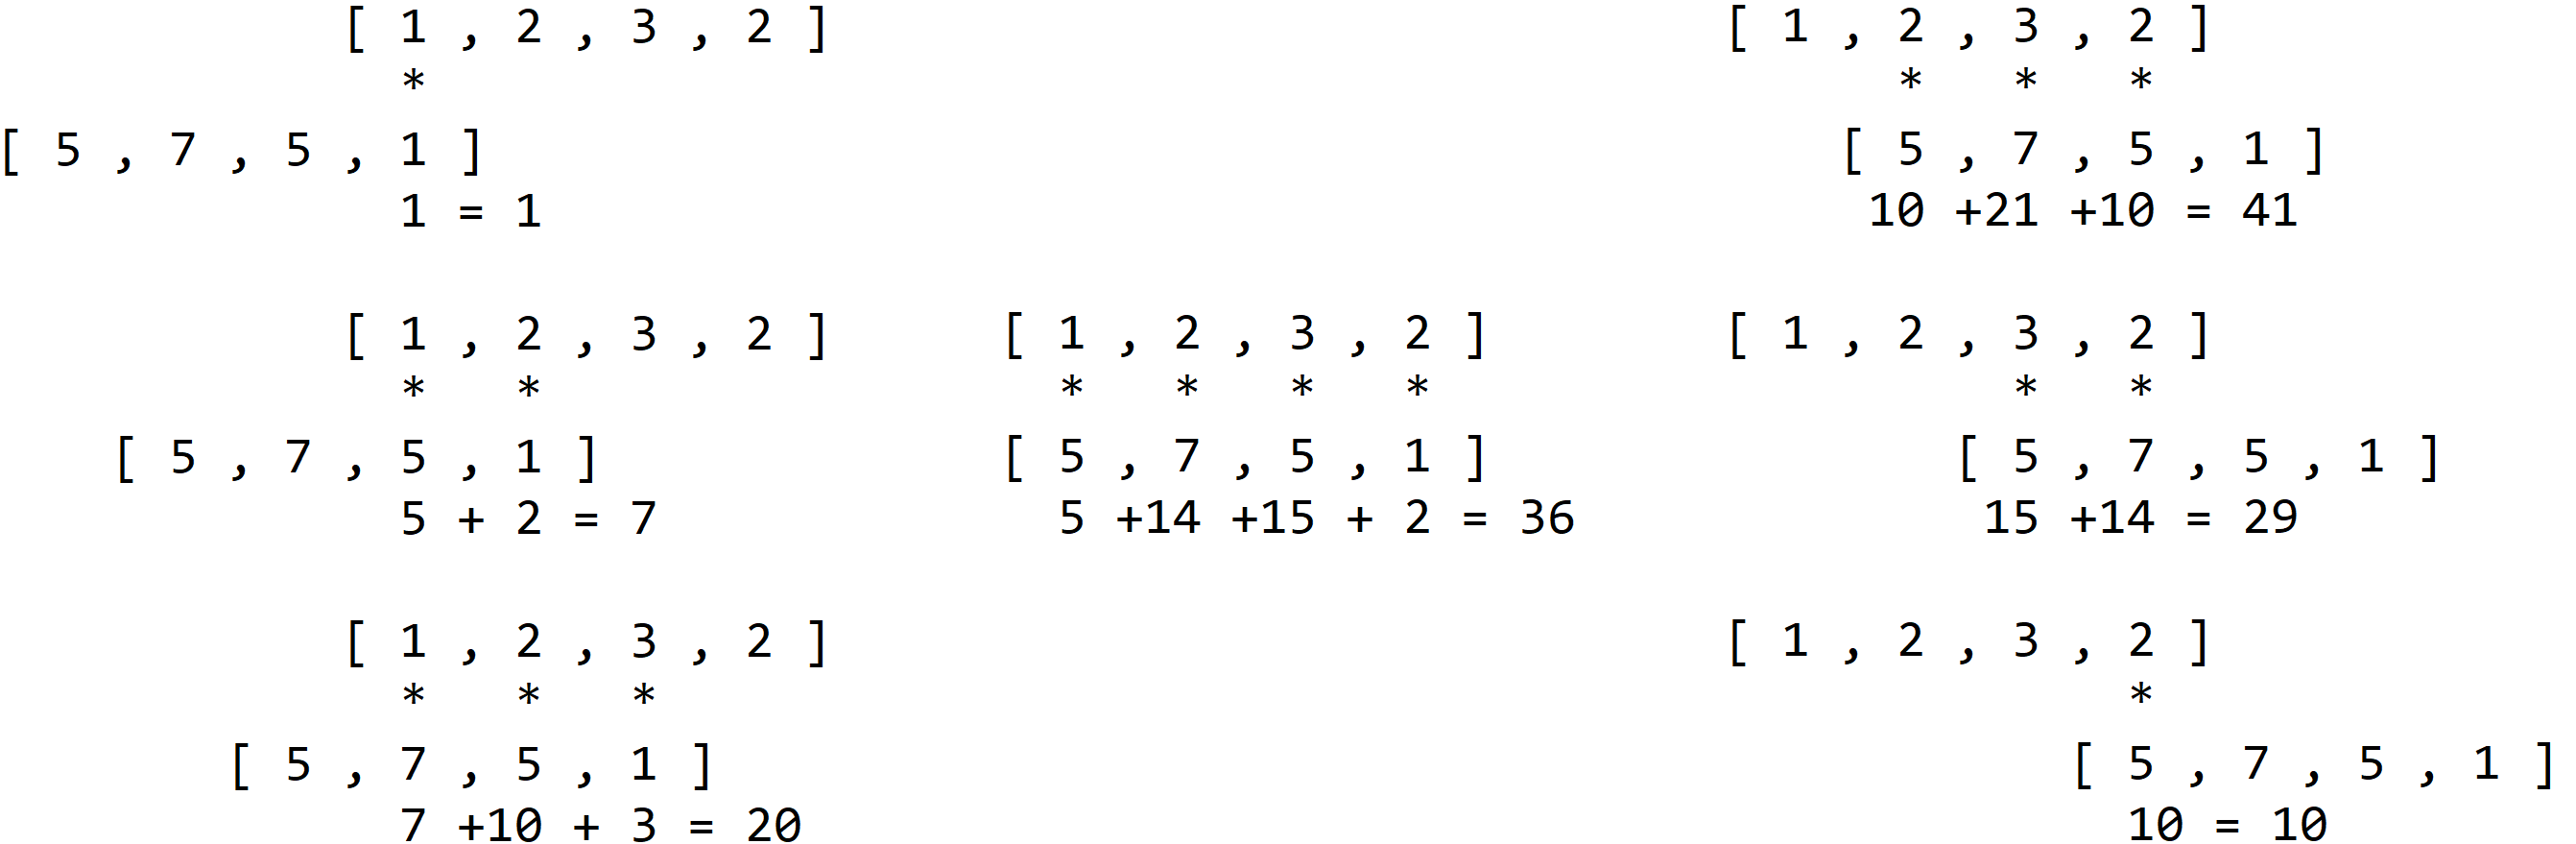
\includegraphics[width=\textwidth]{figures/Korrelation.png}
    \caption{Beispielhafte Darstellung einer Faltung anhand der Folgen $[1,2,3,2]$ und $[5,7,5,1]$. Auf der linken Seite hinter dem Gleichheitszeichen von oben nach unten die Korrelationswahrscheinlichkeiten für die negativen Verschiebungen $\tau=-3$, $\tau=-2$ und $\tau=-1$. Entsprechend in der Mitte bei keine Verschiebung ($\tau=0$) und rechts für die positiven Verschiebungen $\tau=1$, $\tau=2$ und $\tau=3$}
    \label{fig:Korrelation Beispiel}
\end{figure}


Normalerweise müsste für die echte Korrelationswahrscheinlichkeit jede Summe, die einer möglichen Verschiebung zugeordnet ist, durch die Anzahl ihrer aufsummierten Produkte geteilt werden.
Da in diesem Fall die Zeitserien circa 500 Tage umfassen, Korrelationen größer 50 Tagen jedoch nicht beachtet werden, da es sich bei steigender Verzögerung wahrscheinlicher um Zufälle handelt und nur die Korrelationen gezeigt werden sollen, welche mit sehr hoher Wahrscheinlichkeit von der Verschiebung von $\tau = 0$ abweichen, wird hier nicht durch die Anzahl der Produkte geteilt und damit eine leichte Übergewichtung von geringeren zeitlichen Verschiebungen vorgenommen.

\section{Durchschnitt, Farbgebung und Skalierung}\label{sec:Durchschnitt, Farbgebung und Skalierung}
Um schnell verständliche Abbildungen bereitstellen zu können, werden die Werte skaliert und die Farbgebung der Deutschlandkarten derart angepasst, dass das gesamte Farbspektrum abgedeckt wird. Das Farbspektrum reicht gemäß den Farben des Regenbogens von blau über grün zu gelb zu rot. Die niedrigsten Werte werden blau gefärbt.

Die Matrizen werden durch die verwendete Programmbibliothek \glqq{}Matplolib\grqq{} automatisch eingefärbt.


Um die Daten zusammenfassen wird das arithmetische Mittel benutzt. Der Mittelwert entspricht nach \autoref{eq:Mittelwert} der Summe der einzelnen Werte $x_1$, $x_2$, $x_3$ ... $x_n$ geteilt durch ihre Anzahl $n$.
\begin{equation}\label{eq:Mittelwert}
    \bar x = \frac{1}{n}\sum_{i=1}^n x_i
\end{equation}